\section{WC 7/7/25}

\subsection*{Overview:}
This week I began migrating my EPQ report documentation from OneNote to \LaTeX{} in order to produce a more professional and well-structured final report. I also continued to monitor the reception of my EP Artifact: NeuroNote. I continue to receive amazing feedback but will wait until last week before I begin evaluating my project's success

\subsection*{Achievements, Thoughts and Ideas:}
To ensure my report is maintainable as it expands I split the content into a number of 'chapters' (such as Research or Diary) which were folders in my report file and sections which were individual \LaTeX{} pages. With this system in place I started adding a latex file for each diary entry and would create research pieces / prototypes as and when they were referenced. As this was occurring I would nicely migrate my Evaluations, timelines and other more isolated documents into the relevant sections of my report.

Here is an example of a finished diary entry:
\begin{figure}[H]
    \centering
    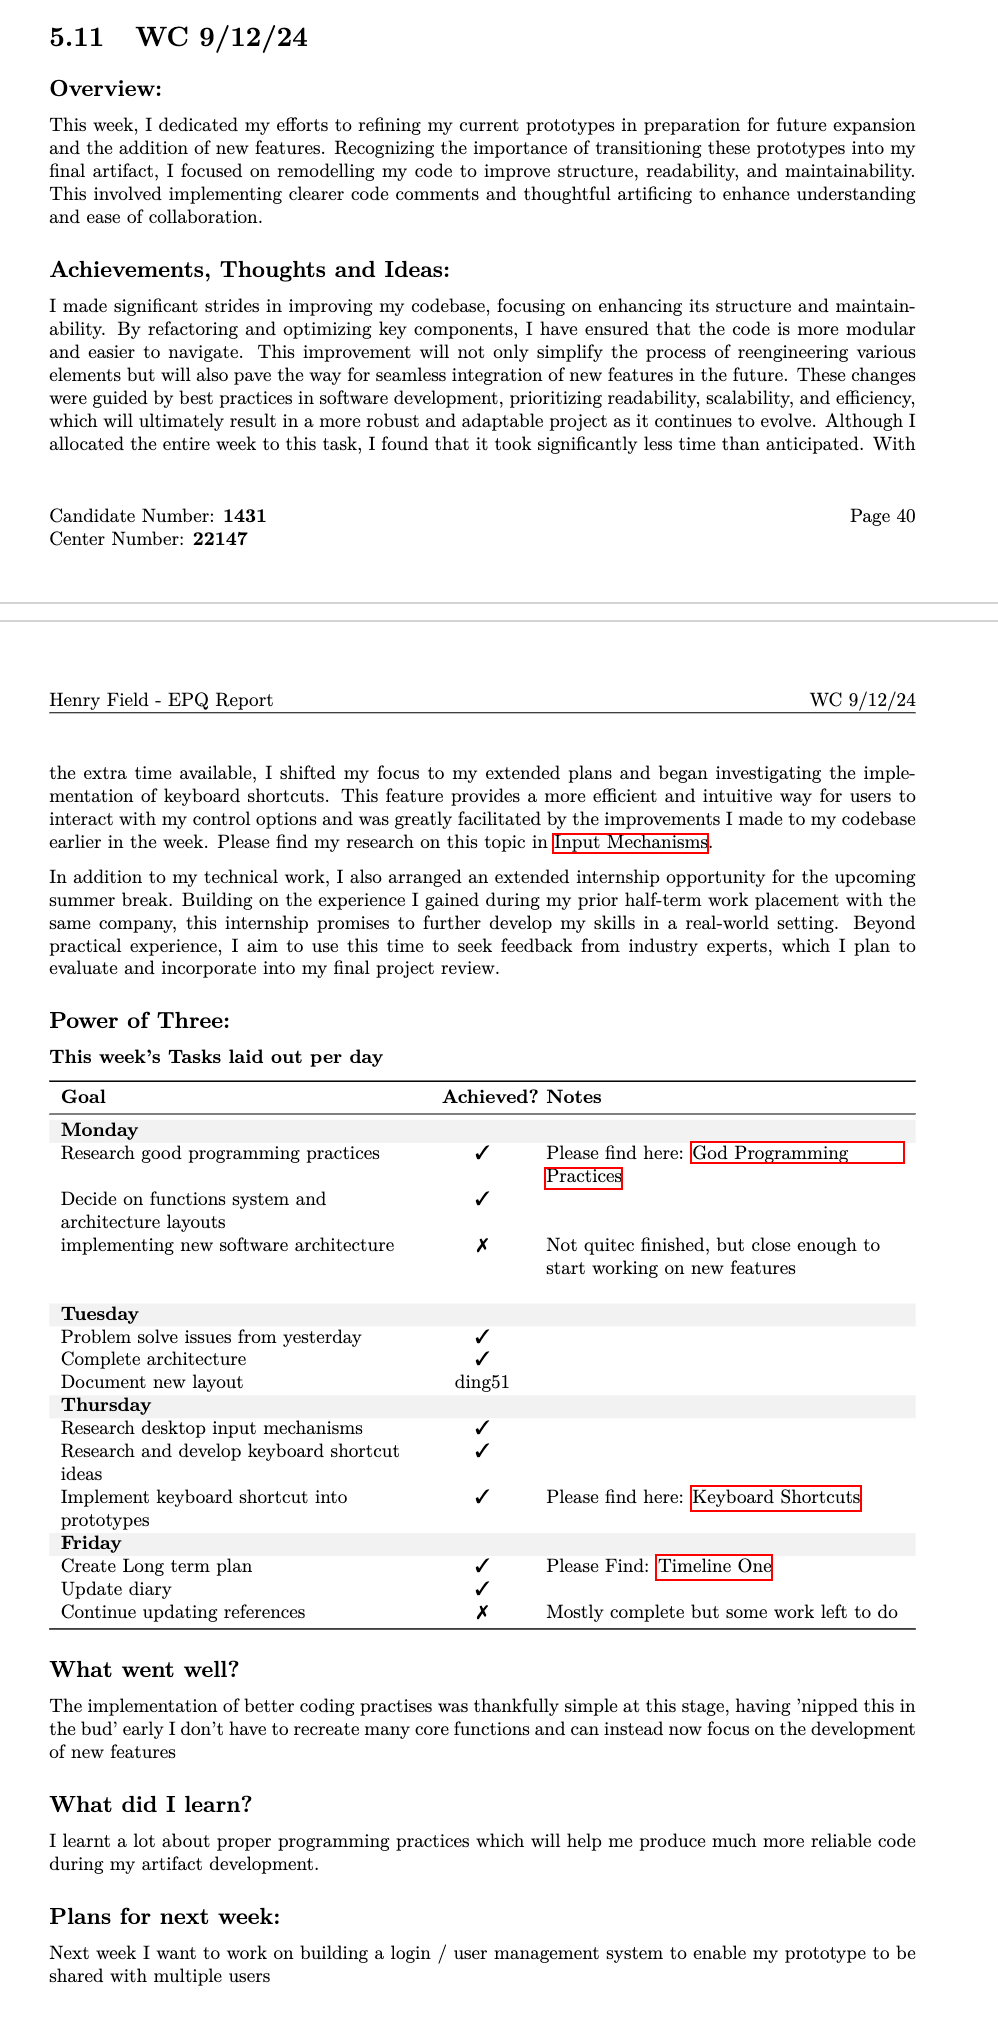
\includegraphics[width=0.6\textwidth]{Diary/36_WC_7-7-25/media/exampleEntry.png}
    \caption{Example of a finished diary entry in \LaTeX{}}
\end{figure}

Although I am pleased with the finished result I soon found that I was duplicating a lot of work for each diary entry and was following the same steps frequently:

\begin{enumerate}
    \item Create a new folder for the diary entry
    \item add a media folder within the folder to store images, code etc
    \item Create a new \LaTeX{} within the folder with the same file
    \item Fill the \LaTeX{} file with the same structure of overview, Achievements etc
\end{enumerate}

To try and maximize my time I experimented with making python scripts that I could call within my code editor, and by providing the date of diary entry or the name of the research piece I could quickly generate the folder structure and \LaTeX{} file. I found this to be a very useful time saver and I have since added this to my skills' evaluation as a new skill. Additionally, I created scripts which would go through the entire Diary/Research/Prototypes folders and automatically organise them into my report complete with table of contents and source links. This was a huge time saver, and I am very pleased with the results.

Here is one of the scripts I wrote to generate a new diary entry:
\inputminted[linenos, tabsize=1, breaklines]{python}{Diary/36_WC_7-7-25/media/ScriptedResearch.py}

So far I have moved around half of my diary entries and there respective media into \LaTeX{} format, the automations I developed have been invaluable in reducing the repetitiveness of the task.

\subsection*{Plans for next week:}
Next week I will continue to migrate my report documentation and will evaluate the reception of my EP Artifact.